\chapter{Introduction}%
\label{chap:intro}
\glsresetall

% \gls, \glspl, \Glspl, \acrlong{cpm}
Technology has been growing exponentially over the last few decades.
The constant evolution of computers, the internet, wireless telecommunication, smartphones, cameras, and other modern technologies are drastically transforming the world we perceive and are improving our standard of living.
If not for the cameras that captured my childhood days through photos and videos as memoirs, the world I grew up in would have been nothing but fiction for the current and future generations.
Nowadays, cameras have become an integral part of our daily lives - be it for taking selfies using our smartphone to post on social media or for collaborating with my colleagues over a video call.
Cameras, as sensors, have also become the "eyes" to perceive the surroundings for modern automotive systems, robots, autonomous systems and manufacturing systems.

\Gls{ibc} systems that use cameras as sensors, are increasingly popular due to their low-cost and high versatility. 
Cameras enable the perception of depth, relative position, geometry, relative distance, colour, and tracking of the object-of-interest. 
As such, \gls{ibc} systems are now an integral part of industrial \glspl{cps}.
\Glspl{cps} refer to a class of modern industrial systems with tight interaction between computation, communication and control elements (the cyber part), and physical processes such as motion, heating/cooling, vibration, wear and tear (the physical part) within these systems.
Designing \glspl{cps} requires an integrative design approach that allows for optimisation coping with the tight coordination between the cyber and the physical components~\cite{lee2008cyber,gunes2014survey,sanislav2012cyber}.
The \gls{ibc} system is compute-intensive and a standalone \gls{ibc} system behaves similar to a \gls{cps}.

This thesis focuses on optimising the design and implementation of \gls{ibc} systems in the resource-constrained \gls{cps} domain.
The case study used throughout this thesis is a \gls{lkas}, though the methods are directly applicable to similar systems in the \gls{cps} domain.
In this introductory chapter, first, the history of the camera and its modern significance are briefly explained.
Second, the context, definition and scope of \gls{ibc} systems are illustrated.
Then, an overview of the state-of-the-art is given and the research challenges with the contributions of this thesis are enumerated. 
After providing an overview of the design and optimization flow elaborated in this thesis, finally, the motivating case study and the thesis outline are detailed.

\section{Evolution of cameras}
"A camera is an optical instrument that captures a visual image.
The camera body has a small hole (the aperture) that allows light through to capture an image on a light-sensitive surface (usually photographic film or a digital sensor). Lenses focus the light entering the camera, and the size of the aperture can be widened or narrowed. A shutter mechanism determines the amount of time the photosensitive surface is exposed to light"~\cite{cameraWiki}.
The invention of the camera has been traced back to the work of Alhazen (Ab\={u} `Al\={i} al-\d{H}asan ibn al-\d{H}asan ibn al-Haytham). Alhazen invented the pinhole camera \emph{camera obscura}, and explained its scientific principles in his magnum opus \textit{Book of Optics} (\textit{Kit\={a}b al-Man\={a}\d{z}ir}) in the 11\textsuperscript{th} century AD~\cite{al2015retrospect}. 
The camera obscura was originally used for viewing solar eclipses instead of looking directly at the sun and damaging the eye.

\begin{figure}[hb]
    \centering
    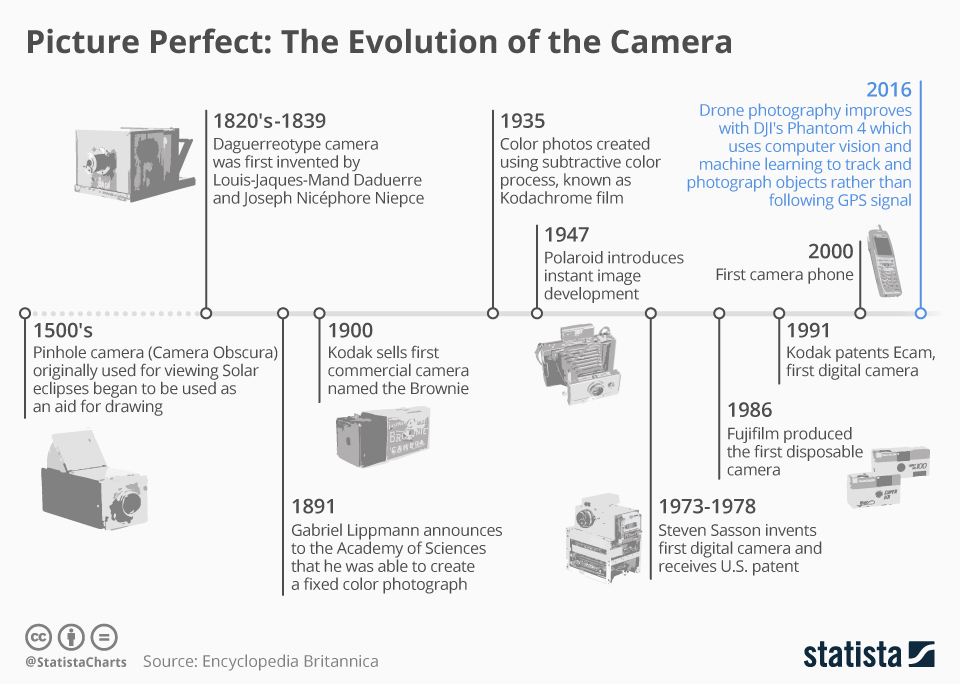
\includegraphics[width=\textwidth]{Figures/camera_timeline.jpeg}
    \caption{The evolution of the camera~\cite{statista2019camera}.}
    \label{fig:CameraEvolution}
\end{figure}

The camera has evolved over the last millennium in technology, functionality and versatility. 
A brief overview of the evolution of the camera (that uses visible light) is illustrated in Fig.~\ref{fig:CameraEvolution}.
Artists used the first pinhole cameras to draw the outline of their paintings from real landscapes.
Then, the cameras were used to preserve memories and store the image information in a physical format.
The landmark moment was the invention of the digital camera, where the image is recreated from the light falling on a \gls{ccd} instead of a photographic film.
The first digital camera was invented by Llyod and Sasson in 1975 and patented in 1978~\cite{lloyd1978electronic}. 
However, at that time, it did not gain the necessary recognition it deserved~\cite{estrin2015Kodak} due mostly to managerial decisions.
One of the reasons for non-acceptance was that it took 23 seconds to record a captured image into a cassette tape (for storage).
The first professional digital \gls{slr} camera was created by Sasson and Hills in 1989 and patented in 1991~\cite{sasson1991electronic}. 
"It had a 1.2 megapixel sensor, and used image compression and memory cards"~\cite{estrin2015Kodak}.

\begin{figure}[ht]
    \centering
    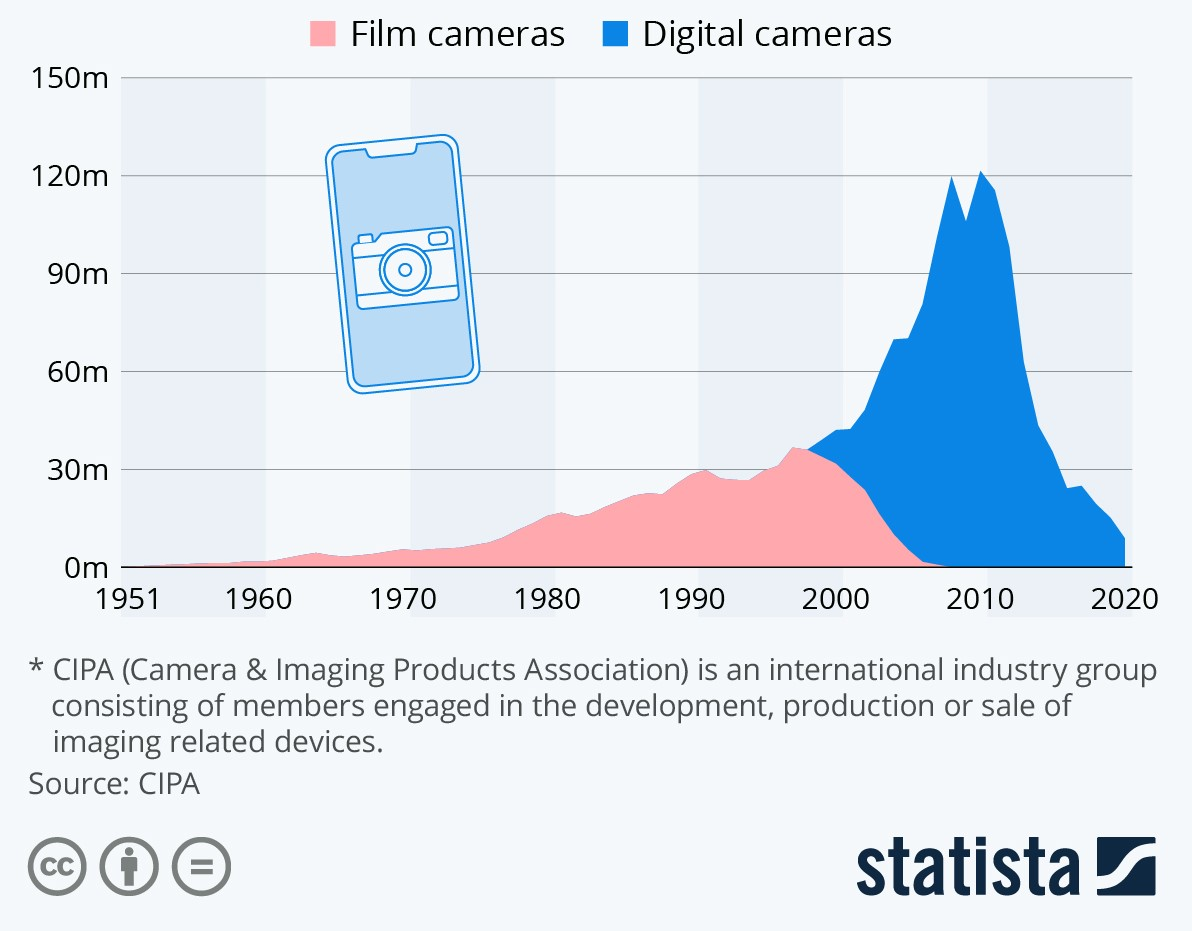
\includegraphics[width=0.7\textwidth]{Figures/camera2.jpeg}
    \caption{Worldwide shipments of photo cameras~\cite{statista2021camera}.}
    \label{fig:CameraSales}
\end{figure}

The invention of the professional digital camera revolutionised the camera market and also increased the global camera market size and revenue. 
The growth of photo camera sales is illustrated in Fig.~\ref{fig:CameraSales}.
Two interesting points to note are: (i) the domination of digital cameras over film cameras that wiped out the normal use of film cameras; and (ii) the drastic decline in sales of digital photo cameras.
The latter is due to the advancements in technology and the integration of high-quality cameras in smartphones and tablets. 
Buying a modern smartphone with a high-quality camera is generally preferred over a single-purpose photo camera. 

\begin{sloppypar}
Advancements in low-cost \gls{cmos} image-sensor technology~\cite{el2005cmos} and Moore's law~\cite{moore1998cramming} enabled the faster integration of cameras in smartphones and modern industrial systems.
Moore's law predicted that the number of transistors in integrated circuits would double every two years, and this has been happening over the last many decades.
This enabled the miniaturisation of the size of the semiconductor component.
Alternatively, many more \gls{cmos} sensors, processors and memories can be densely packed into a semiconductor component of the same size.
This reduced the overall cost and size of the camera, thus enabling the widespread use of cameras in smartphones, laptops, security devices, video surveillance, drones, autonomous systems, modern industrial systems, and so on.
For instance, the latest Samsung Galaxy S21 FE 5G smartphone has four cameras - a 12MP ultra-wide camera, a 12MP wide-angle camera, an 8MP telephoto camera, and a 32MP selfie camera~\cite{samsungS21}.
\end{sloppypar}

\begin{figure}[ht]
    \centering
    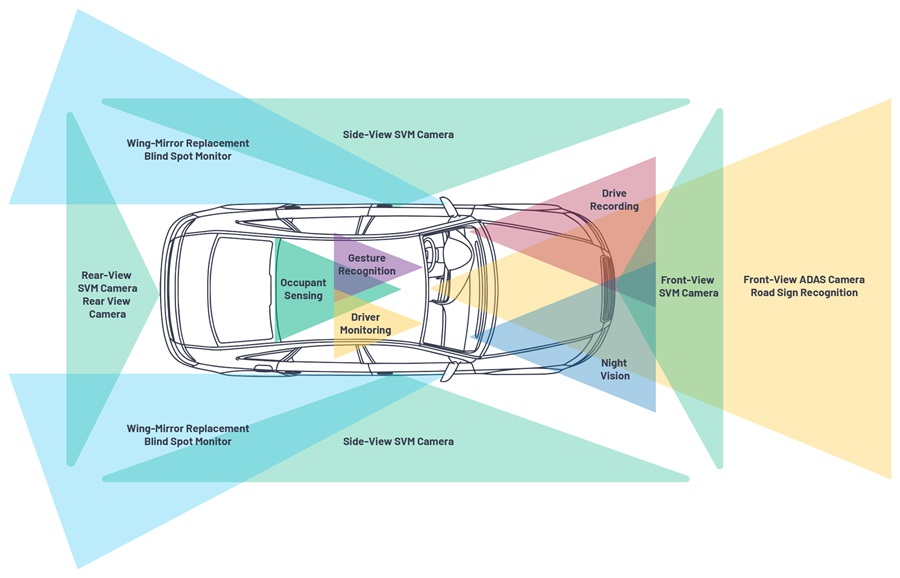
\includegraphics[width=\textwidth]{Figures/295762-fig-01.jpg}
    \caption{Proliferation of cameras in modern vehicles~\cite{triggs2020camera}.}
    \label{fig:CameraProliferation}
\end{figure}

The latest Tesla autopilot system has eight cameras~\cite{tesla}, which are necessary for the three-dimensional perception of the surrounding environment~\cite{elluswamy2021predicting}.
In the automotive domain, there is an immense proliferation of cameras in modern vehicles (illustrated in Fig.~\ref{fig:CameraProliferation}).
According to an industrial report from Yole~\cite{yole19}, the number of cameras in a single vehicle is expected to grow even further. Yole estimates 11 cameras per vehicle by 2024 for functionalities like surround-view, \glspl{adas}, night vision, e-mirror replacement and driver monitoring.
Yole predicts that cameras would also be an integral part of fully autonomous systems.
Additionally, different types of cameras (based on the wavelength of light) are gaining significance for varied purposes, such as hyperspectral cameras~\cite{behmann2018specim}, thermal-imaging cameras~\cite{lee2018analyzing} (using infrared light) and laser imaging (used in lidar sensors~\cite{li2020lidar}). 
Cameras have thus proven to be irreplaceable for modern applications and systems in the coming decades.

\section{Image-based control systems}
Cameras are now an integral part of modern (industrial) systems and are becoming increasingly popular in mixed-criticality systems.
A mixed-criticality system is a system that can execute several applications of different criticality levels - safety-critical, mission-critical and low-critical \cite{burns2013mixed}.
The criticality levels are formally defined, for example, as safety integrity levels in the IEC 61508 standard \cite{bell2006introduction} and \glspl{asil} in the automotive ISO 26262 standard \cite{jeon2011automotive}.
The versatility of the camera sensor allows an image captured by a single camera sensor to be used for multiple mixed-criticality applications.
In the automotive domain, for example, cameras are used to perceive the surrounding environment, enabling safety-critical autonomous driving and use for non-critical applications like drive recording.

\Gls{ibc} systems are a class of data-intensive feedback control systems whose feedback is provided by image-based sensing using cameras as sensors. 
Data-intensive feedback control systems are common nowadays due to advancements in \glspl{cps} \cite{van2018data}.
\Gls{ibc} systems have become popular with the advent of efficient image processing algorithms and low-cost \gls{cmos} cameras with high resolution \cite{corke2017robotics}. 
The combination of the camera and the image-processing algorithm gives necessary information on parameters such as relative position, geometry, relative distance, depth perception and tracking of the object-of-interest. 
This enables the effective use of low-cost camera sensors to enable new functionality or replace expensive sensors in cost-sensitive industries like automotive \cite{corke2017robotics,pendleton2017perception,saidi2018future}.
Applications of \gls{ibc} are found in robotics \cite{corke2017robotics}, autonomous vehicles \cite{elfring2016effective,pendleton2017perception}, advanced driver assistance systems (ADAS) \cite{bengler2014three}, electron microscopes \cite{FEI}, visual navigation \cite{chakraborty2016compensating} and so on.

The popularity of modern \gls{ibc} systems can be attributed to 
\begin{itemize}
    \item the impact of Moore's law \cite{moore1998cramming} and the constant breakthroughs in semiconductor manufacturing technology. This enabled the availability of powerful multiprocessors at relatively low cost and size, and also paved the way for the miniaturisation of \gls{cmos} cameras.
    \item the availability of low-cost high-resolution \gls{cmos} cameras with good quality and small size.
    \item the versatility of the camera images and the breakthroughs in \gls{ai} technology and deep-learning algorithms \cite{lecun2015deep}. Using deep-learning methods and algorithms, a multitude of features can be efficiently extracted from camera images and used for a variety of mixed-criticality applications.  
    \item the industrial adoption of heterogeneous platforms and the breakthroughs in \glspl{gpu} and \glspl{npu}. Examples of such developments are Tesla's \gls{fsd} computer \cite{talpes2020compute} and NVIDIA's Drive AGX platform \cite{nvidiadrive}. 
   The  \gls{fsd} computer is based on a \gls{soc} that integrates industry standard components such as \glspl{cpu}, \gls{isp}, \glspl{gpu}, and \glspl{npu}.
\end{itemize}

\begin{figure}[htb]
\centerline{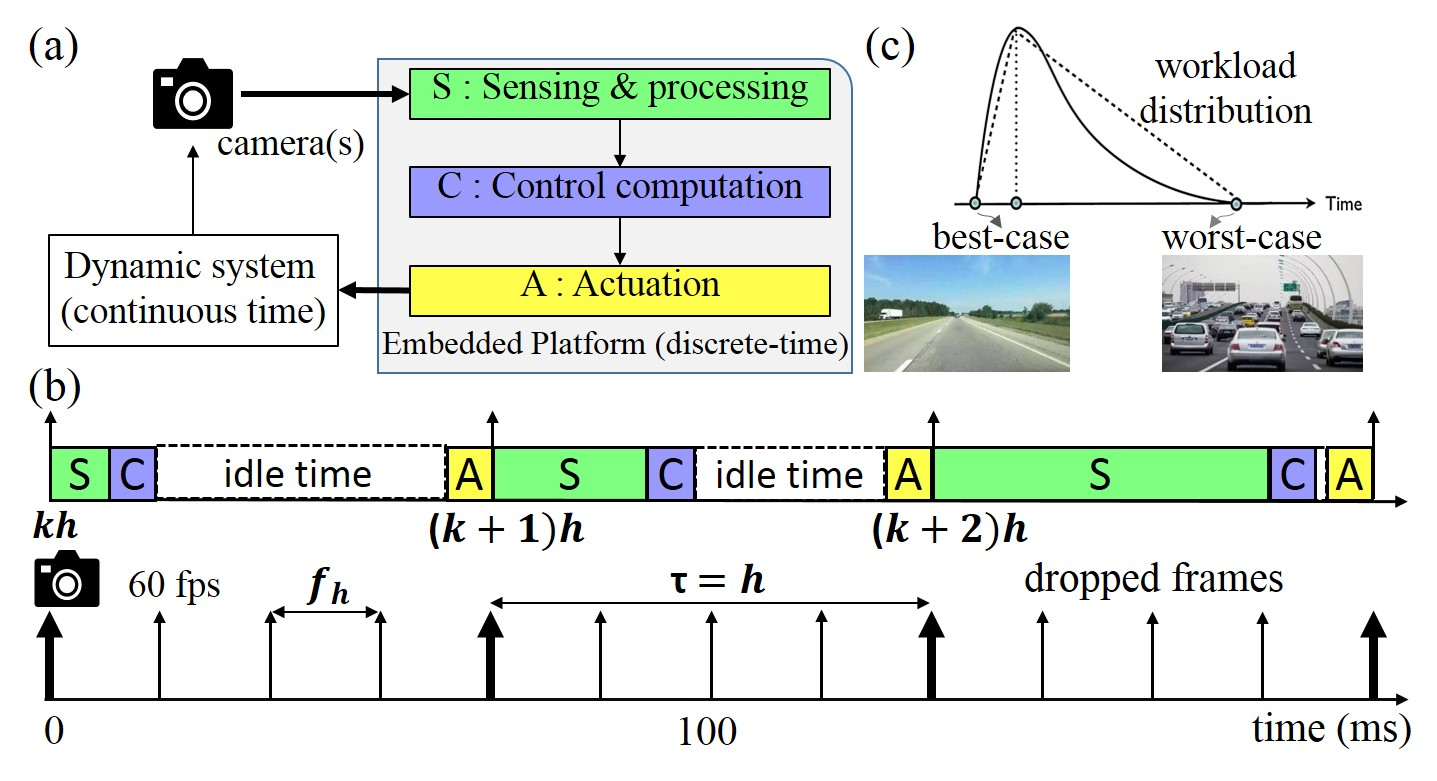
\includegraphics[width=\textwidth]{01_intro/images/ibc_intro.jpg}}
\vspace{-1ex}
\caption{An \acrfull{ibc} system: (a) block diagram; (b) Gantt chart for a typical \gls{ibc} implementation; (c) workload variations captured as a distribution. In the context of the thesis, workload refers to the image workload (unless specified differently). Image workload refers to the number of features in the image that should be processed. For example, more features in an image typically implies a higher workload.}
\label{fig:ch1_ibc_intro}
%\vspace{-2em}
\end{figure}

In this thesis, the focus is on \gls{ibc} systems that are functionally critical and on feedback control systems whose state is measured by the image-based sensing and processing, i.e., state feedback.
The case study of an automotive \gls{lkas} system is used to explain the concepts and results of this thesis.
A typical \gls{ibc} system is illustrated in Fig. \ref{fig:ch1_ibc_intro} (a).
A camera captures image frames at a pre-defined constant frames per second $\fps$, i.e., the frame rate, from the dynamic system environment (with the camera frame-arrival period $\fh$ $=\frac{1}{\fps}$).
An \gls{isp} processes the RAW camera image frames in the Bayer domain and converts it to the standard RGB image format, e.g. JPEG. 
Then, a compute-intensive image-processing algorithm processes the image frames to detect features in the image such as objects, traffic signs and lanes.
These features are then used to compute the states of the system, such as relative position and distance \cite{corke2017robotics}.
A controller computes the control input for actuation (e.g., change in direction) using the computed states.
The actuation task applies the computed control input to the \gls{ibc} system.

A typical feedback control implementation sequentially and
periodically (with sampling period $h$) executes the sensing and processing task (S), control compute task (C) and the actuating task (A) (as illustrated in Fig. \ref{fig:ch1_ibc_intro} (b)).
In an \gls{ibc} system, the sensing task may have a long, variable execution time and incur a long sensing delay. 
Variability in execution time may occur due to variation in image-processing workload and/or in the platform load caused by other applications.
The key \textit{challenge} is to deal with this \textit{high dynamic computation demand while guaranteeing performance and meeting safety requirements} such as stability.
A long variable processing delay results in dropping some camera frames from processing. 

These variations can be captured statistically using a probability distribution \cite{adyanthaya2014robustness} (illustrated in Fig. \ref{fig:ch1_ibc_intro} (c)).
It is interesting to note that this delay distribution is platform-dependent.
Platform-related parameters - for instance, number of processing cores, processor clock speed, memory, and communication bandwidth - have a direct impact on the observed delay. 
A long worst-case sensing delay leads to a long sensor-to-actuator delay $\tau$ (the time between the start of a sensing task and the end of the corresponding actuation task) and thus results in degraded control performance \cite{sharkey1996delays,aastrom2013computer}.

In this thesis, we develop approaches to cope with a long variable sensing delay exploiting the benefits of a multiprocessor platform and the application-specific \gls{ibc} system characteristics.
The platform-aware aspects explored in this thesis that exploit the benefits of a multiprocessor platform are - application parallelisation and pipelining of the control loop.
Parallelisation refers to executing sensing subtasks in parallel and thereby reducing the delay compared to the sequential implementation. 
Pipelining refers to the pipelined execution of the control loop over multiple processing cores thereby reducing the effective sampling period (the time between the start of two successive sensing tasks).
The two application-specific characteristics we exploit are - the image workload variations and approximate computing. 
Image workload variations occur due to the variations in the number of features in the captured images and the platform load. 
Approximate computing trades off accuracy in the signal processing for gains in response time and energy.

\section{Implementation platforms}
%\label{sec:implementation platforms}

A platform refers to the combination of hardware resources (computation, communication, and memory) and the software (tasks, messages, mapping and scheduling) required to deploy an algorithm/application on the hardware effectively.
The execution time of tasks - sensing and processing (\taskS), control compute (\taskC), and actuation (\taskA) - of an \gls{ibc} system is dependent on the platform configuration.
The relatively straightforward way to reduce the long sensing delay is to have a processor with a high clock speed. 
However, this increases the cost of the processor. Moreover, the scaling of clock speed has reached its limits because of physical constraints in chip manufacturing and operation.
Another option to cope with long sensing delay is to have a platform with multiprocessor capabilities that enable concurrent parallel and pipelined execution of tasks.
A multiprocessor platform is economical due to the impact of Moore's law and is common nowadays.

In this thesis, two kinds of multiprocessor platforms are considered for the \gls{ibc} system implementation.
First, a \gls{compsoc} platform~\cite{hansson2009compsoc} is considered.
The \gls{compsoc} platform offers a composable and (timing) predictable implementation for the designer. 
The results of this thesis can be effectively applied to such predictable platforms without any adaptation.
Second, state-of-the-art industrial platforms are considered.
Predictability and composability are usually not offered in an industrial platform. 
We adapt our design approach for the industrial platforms NVIDIA Drive PX2 and NVIDIA AGX Xavier~\cite{nvidiaAGX} to demonstrate its applicability in an industrial context.
Our design approach is also applicable for more recent industrial platforms like the Tesla \gls{fsd} computer~\cite{talpes2020compute} and NVIDIA Drive AGX~\cite{nvidiadrive}.

\begin{figure}[t]
\centerline{
    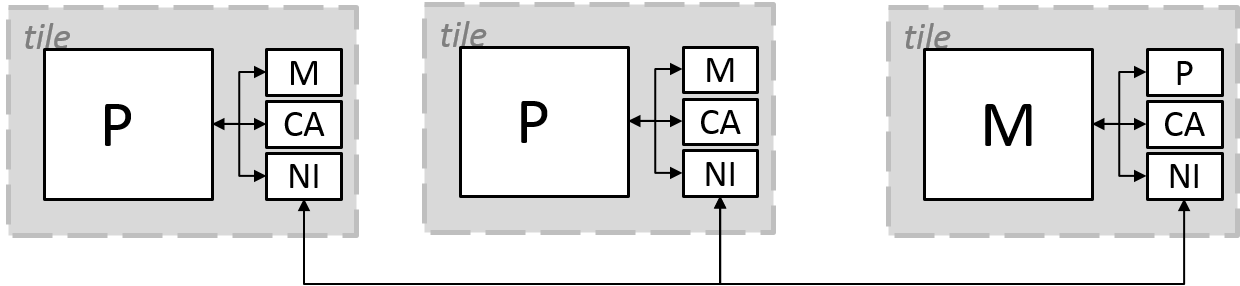
\includegraphics[width=0.8\textwidth]{01_intro/images/mpsoc_wo_index.png}
    }
    \caption{A \gls{compsoc} platform with two processor tiles and a memory tile connected through a \gls{noc}.}
    \label{fig:mpsoc}
    %\vspace{-2em}
\end{figure}

\subsection{\Gls{compsoc}}
\label{sec:compsoc}
\gls{compsoc} offers a tile-based architecture~\cite{stuijk2007} (see Fig.~\ref{fig:mpsoc}). Each tile has a processor $P$, memory $M$, communication assist $CA$ and network interface $NI$. 
Each processor tile has a microblaze processor, the memory tile contains an external memory interface, e.g., \gls{dram}, and the \gls{noc} provides interconnection between the tiles.
The platform is predictable with tight bounds on \glspl{wcet} of tasks and composable so that applications sharing the platform do not interfere with each other. 
A scheduler performs (re)configuration and time-triggered task execution. 

\begin{figure}[ht]
\centerline{
    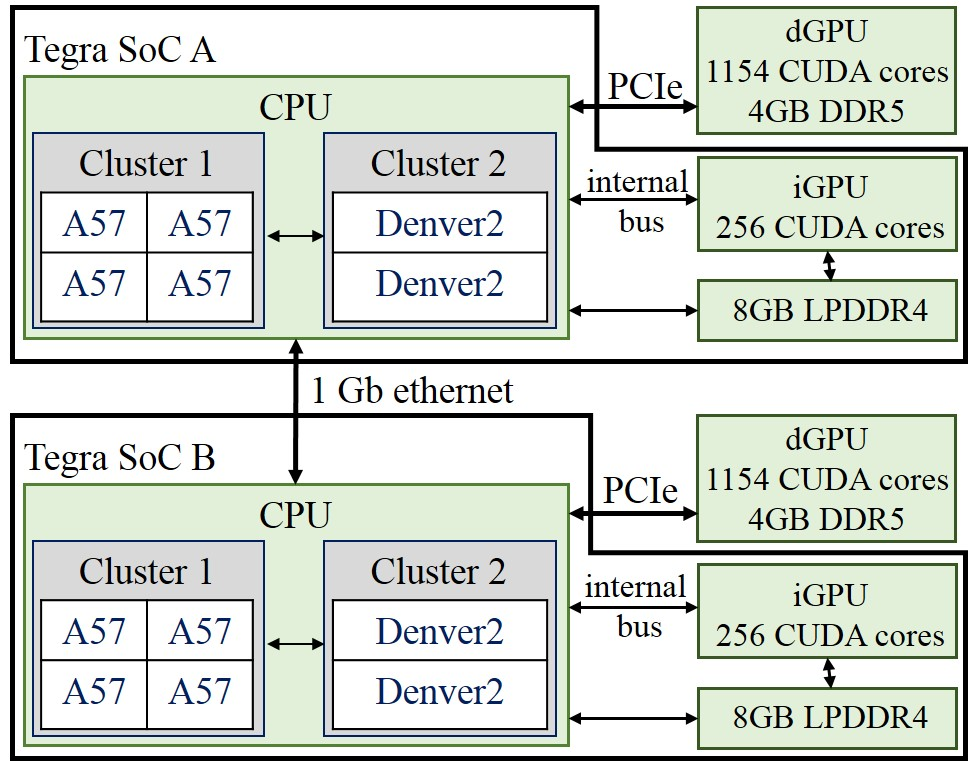
\includegraphics[width=0.65\textwidth]{01_intro/images/drive_platform.jpg}
    }
    \caption{NVIDIA Drive PX2 platform structure. LPDDR4 and DDR5 are the memory blocks. Each CPU cluster also has internal instruction and data memory (not shown in the graph).}
    \label{fig:drive_platform}
    %\vspace{-2em}
\end{figure}
\subsection{NVIDIA Drive PX2}
\label{sec:nvidia_px2}
The NVIDIA Drive PX2~\cite{nvidiadrive} platform consists of two Tegra \glspl{soc} that communicate to each other via ethernet. Each Tegra \gls{soc} has two \gls{cpu} clusters (see Fig.~\ref{fig:drive_platform}). One
cluster contains four ARM Cortex A57 cores and the other
contains two NVIDIA Denver2 cores. The clusters are connected
through a high-performance network interconnect. Each of the
Tegra \glspl{soc} also has two \glspl{gpu} -
an \gls{igpu} and a \gls{dgpu} with maximum clock rates of 1.27 and 1.29 GHz respectively. The \gls{igpu} has 256 CUDA cores and the \gls{dgpu} has 1154 CUDA cores. The \glspl{gpu} are accessed via the respective \glspl{cpu} in the \gls{soc}. The Ubuntu 16.04 LTS \gls{os} runs on the \gls{cpu} platform. 

\subsection{NVIDIA AGX Xavier}
\label{sec:nvidia_agx}
The NVIDIA AGX Xavier platform (illustrated in Fig.~\ref{fig:nvidia_platform}) consists of a Xavier \gls{soc} and other components explained in~\cite{nvidiaAGX}.
The \gls{cpu} complex consists of four heterogeneous dual-core NVIDIA Carmel \gls{cpu} clusters based on ARMv8.2 with a maximum clock frequency of 2.26GHz. 
The \gls{gpu} with a maximum clock frequency of 1.37GHz is accessed via the \glspl{cpu} in the \gls{soc}. The Ubuntu 18.04 LTS \gls{os} runs on the \gls{cpu} platform.
\begin{figure}[t]
\centerline{
    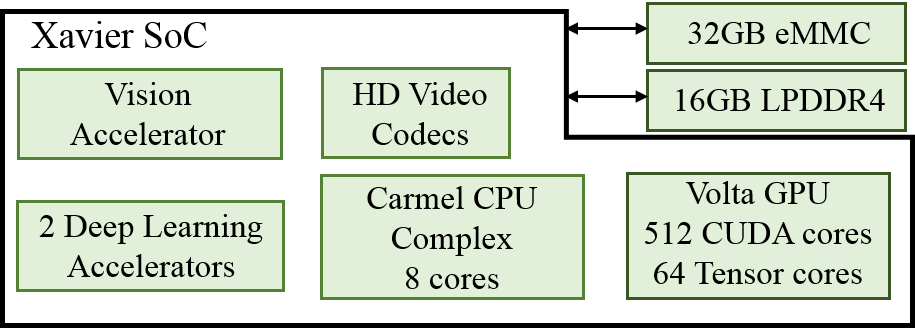
\includegraphics[width=0.65\textwidth]{01_intro/images/platform.png}
    }
    \caption{NVIDIA AGX Xavier platform block diagram. LPDDR4 and eMMC are the memory blocks. Each \gls{cpu} cluster also has internal instruction and data memory (not shown in the graph).}
    \label{fig:nvidia_platform}
    %\vspace{-2em}
\end{figure}

\section{State-of-the-art}
\label{sec:sota}
This thesis explores techniques to cope with the long variable sensing delay by considering application-specific \gls{ibc} system characteristics and exploiting the benefits of multiprocessor platforms. Effectively handling the long variable sensing delay helps to optimise \gls{ibc} system performance while guaranteeing \gls{ibc} system stability.
State-of-the-art methods do not fully exploit the \gls{ibc} system characteristics and advantages of the multiprocessor platforms for optimising the sensing delay. The \gls{ibc} system sensing delay is also variable with a significant degree of variation between the best-case and worst-case delay due to application-specific image-processing workload variations and platform characteristics. A long variable sensing delay degrades system performance and stability. A tight predictable sensing delay is required to optimise the \gls{ibc} system performance and to guarantee the stability of the \gls{ibc} system. Analytical computation of sensing delay is often pessimistic due to image-dependent workload variations or challenging platform timing analysis.

Relevant literature deals with the following questions: 
\begin{itemize}
    \item What are the relevant overall design approaches for such embedded control problems? 
    \item What are the relevant \gls{ibc} system modelling and analysis techniques?
    \item What are the techniques for \gls{ibc} system design to deal with long delays in a feedback control loop?
\end{itemize}

\noindent\textbf{Design approaches:} An \gls{ibc} system is often designed based on the \emph{separation-of-concerns} principle between the control theory and embedded systems disciplines~\cite{arzen2000introduction,saidi2018future}.
Co-design of control and scheduling is another design paradigm explored in the literature~\cite{cervin2003does}.
The emphasis is on platform-based design methods that take into account platform resource constraints while designing the controller~\cite{arzen2000introduction,goswami2013multirate}.
Contract-based design~\cite{sangiovanni2012taming} is a platform-based design paradigm for cyber-physical systems where the interactions between control theory and embedded design are defined based on contracts.

From the embedded-systems discipline, a system-scenario-based design approach~\cite{gheorghita2009system} is proposed where different behaviours (scenarios) of an application are explicitly considered to avoid over-dimensioning or sub-optimal performance due to worst-case design. 
Identifying, characterising and modelling these scenarios and dealing with the runtime scenario transitions are specific for each application and generally not trivial.
In this thesis, we combine scenario-based and platform-based design methods into a coherent \gls{spade} approach for \gls{ibc} system design and implementation.
\\[1ex]
\noindent\textbf{\gls{ibc} system modelling:} Model-based design~\cite{lee1998framework,thiele2000real} approaches focus on designing applications based on abstract models of application and platform such that the implementation is guaranteed to behave with predictable performance. 
Numerous \gls{moc} are available in literature~\cite{theelen2006scenario,stuijk2010predictable, ChakrabortyKT03, DavisBBL07}. 
The approaches in this thesis do not depend on a specific \gls{moc}.
They need a \gls{moc} that can capture the dynamic behaviours (scenarios) of the application, can analyse timing and has support for platform-aware mapping analysis. 
\\[1ex]
\noindent\textbf{\gls{ibc} system design - control engineering perspective:}
The main challenge in designing an \gls{ibc} system is to cope with the long sensing delay.
Control engineers tackle a long delay using advanced state estimation~\cite{wang2014multirate}, robust design~\cite{kawamura2012robust}, predictive control~\cite{macesanu2014time}, observer-based~\cite{van2018data} methods, and multi-rate
sampling~\cite{fujimoto2003visual} methods. 
These methods rely heavily on the system model and are vulnerable to modelling errors with longer delays.
Also, control engineers typically design an \gls{ibc} system considering the worst-case image workload~\cite{saidi2018future} and do not explicitly consider the platform constraints.
In literature, workload variations are typically considered only for sequential \gls{ibc} implementation~\cite{fontantelli2013optimal} and not for parallel and pipelined implementations~\cite{medina2019designing},~\cite{krautgartner1998performance}. 
In~\cite{medina2019implementation}, pipelining is considered along with variable delay.
However, these approaches do not consider system nonlinearities, i.e., the variations in system dynamics, and constraints imposed on the system variables, which can be crucial when considering a practical implementation.  
\\[1ex]
\noindent\textbf{\gls{ibc} system design - embedded systems perspective:}
Embedded systems engineers aim to reduce processing delay and period by parallel implementations of the algorithms using heterogeneous multiprocessor platforms having specialised hardware such as GPUs~\cite{agrawal2014gpu} and FPGAs~\cite{kestur2012emulating}. 
Pipelined control~\cite{krautgartner1998performance,medina2019designing} is another approach targeting homogeneous multiprocessor implementations that reduce the effective sampling period without changing the processing delay.
Inter-frame dependencies, i.e. the data or algorithmic dependencies between consecutive frame processing, e.g. due to video coding~\cite{li2015lagrangian} or visual tracking~\cite{smeulders2013visual}, and resource sharing between pipes, which are crucial aspects for a practical pipelined \gls{ibc} system implementation, are not explicitly considered in the literature.
Additionally, we observe that an integral approach to pipelined parallelism can provide immense benefits to the \gls{ibc} system design and implementation. However, such an integral approach is lacking in literature. 
\\[1ex]
\noindent\textbf{\gls{ibc} system design - approximate computing perspective:}
Approximate computing is another technique that can help reduce the processing delay by trading off computation accuracy for speed. 
Approximations reduce the compute workload across algorithm, architecture and circuit levels. Commonly used algorithmic approximations are computation skipping \cite{comp_skip}, precision scaling \cite{precision_scaling} and replacing error-resilient compute-intensive functions with neural networks \cite{nn_invoke}. A learning approach to design \glspl{isp} for new camera systems is proposed in \cite{learning_isp}. At the architecture level, research efforts have focused on both approximating general-purpose processors\cite{ProACt} as well as domain-specific accelerators \cite{sde}. At the circuit level, research efforts focus on manual design techniques for adders and multipliers \cite{approx_maual}, as well as automated methodologies for designing energy-efficient approximate circuits \cite{sde2}.

Approximation benefits in a camera-based biometric security system, using an iris recognition application, is showcased in \cite{8342029}. An approximate smart camera system is introduced in \cite{araha}, using camera resolution scaling, reducing memory refresh rate and computation skipping. An approximate \gls{isp} pipeline tuned for computer-vision algorithms is designed in \cite{buckler}, by skipping selected \gls{isp} stages. An algorithm-hardware co-designed system is showcased in \cite{euphrates}. 
However, these approximation techniques do not consider a closed-loop feedback system. Approximation decisions in a closed-loop system have quality implications at a later point in time. Optimising a system while accounting for the temporal approximate behaviour is not explored in any of the mentioned work.

\section{Research challenges and contributions}
\label{chap:challenges}
\begin{quote}
\centering
The primary research question addressed in this thesis is:\\ \textbf{How to cope with the long variable sensing delay in an \gls{ibc} system?}
\end{quote}
This thesis deals with challenges to cope with the long variable sensing delay in an \gls{ibc} system and the scientific contributions are broadly classified into two directions -- exploitation of the benefits of the multiprocessor platforms through a platform-aware design and exploitation of the application-specific \gls{ibc} system characteristics. 

 In this context, along the first line of research, we exploit the benefits of the multiprocessor platforms through application parallelisation and pipelining of the control loop. 
 The approaches proposed in this thesis maximise the \gls{qoc} of the controller implementation for a given multiprocessor platform allocation.
In the following, we outline the three scientific contributions related to parallelisation, pipelining and pipelined parallelism.
\\[1ex]
\noindent
\textbf{Contribution 1 (\Gls{spade} flow for \Gls{ibc} system design considering parallelisation):}
Parallelisation refers to executing sensing subtasks in parallel and thereby reducing the delay compared to the sequential implementation considered before. A parallel implementation is possible when multiple cores are allocated for the sensing algorithm. 
It is, however, limited by the degree of parallelism of the sensing algorithms. The state-of-the-art literature related to parallel implementation for an \gls{ibc} system does not consider workload variations which is crucial for maintaining optimal closed-loop performance or \gls{qoc}, as already explained. Moreover, a parallel implementation in an \gls{ibc} system is highly influenced by platform-specific parameters such as camera frame-rate, number of available cores and so on. At the end, these design aspects lead to the two important control design parameters --  sampling period and delay. Starting with a given, often pessimistic, sampling period and delay, like what can be noticed in the state-of-the-art \cite{krautgartner1998performance}, the overall design often leads to a low \gls{qoc}.

In this thesis, first, we introduce the \gls{spade} approach for parallel implementation. The \gls{spade} approach uses a formal model-of-computation -- dataflow -- for the entire \gls{ibc} system including sensor processing. This enables us to model workload variation as well as platform-specific design parameters that are crucial for design optimality of a \gls{ibc} system. The contribution of this thesis concerning this case is the relation between dataflow timing analysis and control timing parameters to obtain a tight predictable sensing delay considering implementation constraints.
The image workload variations are captured in workload scenarios and modelled using a \gls{sadf}. 
Then, workload scenarios are mapped to the given platform allocation considering the platform constraints such as the camera frame rate and the number of available cores.
Mapping an \gls{sadf} results in a binding-aware graph. 

In this thesis, we relate the latency and throughput of the binding-aware graph to the delay and sampling period of the controller design. Our approach enables a scenario- and platform-aware design and optimisation of the \gls{ibc} system.
Our approach exploits frequently occurring workload scenarios to optimise control performance.
During controller design, we then optimize performance and guarantee stability by identifying appropriate system scenarios and by designing a switched controller that switches between those scenarios.
The initial proposed approach assumes that the platform is predictable, i.e., the \gls{wcet} of the sensing algorithm for the same image input is bounded and predictable over multiple executions on the platform. 
However, the execution times cannot be bounded for industrial platforms. 
In this thesis, we also show how we can adapt our \gls{spade} approach for parallelisation for an industrial platform where we propose to use frequently occurring task execution times instead of \gls{wcet}.

The first contribution has been published in:
\begin{itemize}
    \item \bibentry{mohamed2020scenario}.
    \item \bibentry{mohamed2018optimising}.
\end{itemize}
With respect to the state of the art, this thesis proposes the first formal model-based design framework for the \gls{ibc} system co-design that relates dataflow analysis and controller design. 
The \gls{spade} approach brings together dataflow and control formalisms in the same framework.
This relation allows to bring in the optimisation techniques from the dataflow domain into the control timing parameter optimisation.
The proposed \gls{spade} approach also makes a step forward towards real-life implementation by detailing how the flow can be adapted for industrial platforms. Both academic and industrial platforms could implement the \gls{spade} approach. \gls{sil} and \gls{hil} simulation results validate our claim.
\\[1ex]
\noindent
\textbf{Contribution 2 (Extending the \gls{spade} flow considering pipelining for \gls{ibc} system design):}
Pipelining refers to the pipelined execution of the control loop over multiple processing cores. It is an alternative to exploit the availability of multiple cores on the platform to address the challenge of long delay in an \gls{ibc} system. In an \gls{ibc} system, a pipelined implementation implies the start of processing a new camera frame while one or more frames are still being processed. In essence, this increases the processing throughput of the frames, which reduces the closed-loop sampling period $h$ (the time between the start of two successive sensing tasks). Although such implementation does not reduce the sensing delay, a shorter sampling period opens the door for achieving a higher \gls{qoc} with an appropriate controller design. 

Given that multiple frames are processed simultaneously, a crucial aspect are the inter-frame dependencies that some of the sensing algorithms might impose. Inter-frame dependencies refer to the data or algorithmic dependencies between consecutive frame processing, e.g., due to video coding \cite{li2015lagrangian} or visual tracking \cite{smeulders2013visual}. Moreover, for a real-life implementation, it is crucial to consider system nonlinearities and constraints
on system variables. System nonlinearities refer to the variations in system dynamics, and constraints need to be imposed on the system variables. For example, the maximum steering angle of the Udacity self-driving car is set to +/- 25 degree \cite{tian2018deeptest} and the vehicle velocity is kept constant for the simulations in \cite{kosecka1997vision}. While pipelined implementations for the \gls{ibc} system is considered in the state-of-the-art as potential direction \cite{medina2019designing}, \cite{krautgartner1998performance}, the existing approaches do not consider several key practical aspects needed for their real-life adoption. 

As a contribution, this thesis presents an extended \gls{spade} approach with an adaptive predictive control formulation based on linear parameter-varying (LPV) input/output (I/O) models for a pipelined multiprocessor implementation of \gls{ibc} systems while considering workload variations, inter-frame dependencies, system nonlinearities and constraints, and thus makes a step forward towards real-life adoption. The inter-frame dependencies are characterised using the platform constraints - camera frame rate and the number of available cores, and the control timing parameters - delay and sampling period. 

The second contribution has been published in:
\begin{itemize}
    \item \bibentry{mohamed2020adaptive}.
\end{itemize}
The state-of-the-art pipelined multiprocessor IBC implementation approaches do not consider inter-frame dependencies, system nonlinearities and constraints on system variables. This thesis proposes a \gls{mpc} formulation that consider these aspects and makes a step forward towards real-life adoption. The simulation results and discussions validate our claim.
\\[1ex]
\noindent
\textbf{Contribution 3 (Extending the \gls{spade} flow considering pipelined parallelism for \gls{ibc} system design\footnote{The \gls{spade} flow controller design is open sourced and can be accessed on github: https://github.com/sajid-mohamed/SPADeControlDesign}):}
In an \gls{ibc} system, a long variable sensing delay results in a long sampling period and a long delay from the controller viewpoint. To deal with them, modern multiprocessor \gls{ibc} implementations consider either parallelisation of the sensing task or pipelining of the control loop. In a pipelined implementation, the sampling period is shortened while the delay remains long. Such implementation does not require knowledge of the internal processing structure of the sensing workload. The benefit of such methods is restricted by the platform parameters such as number of available cores and camera frame-rate. On the other hand, in a parallelised implementation, the delay is shortened allowing for a shorter sampling period. This line of approaches require computational insight (i.e., model-of-computation) of the sensing task for a parallelised implementation. Similar to the pipelined case, the benefits of parallelization methods are restricted by the number of available cores and the degree of parallelism present in the sensing algorithms.  The impact of both parallelisation and pipelining together on the \gls{qoc} of \gls{ibc} systems is not explored in the literature while it is rather obvious direction given their complimentary nature. 

This thesis proposes a model-based design method for multiprocessor \gls{ibc} implementation, considering both parallelisation and pipelining together. It presents model transformations for modelling, analysis
and mapping \gls{ibc} systems using \gls{sadf}. The model transformations allow to relate the dataflow timing analysis to the control timing parameters and to optimise the mapping while considering pipelining and parallelism together.
In this thesis, the particular problem we address is: For a given platform allocation, what is the optimal degree of pipelining and degree of parallelisation required to maximise the \gls{qoc}?
A unified \gls{spade} algorithm is proposed that takes into account image-workload variations, inter-frame dependencies and platform constraints.
The application is efficiently modelled and analysed using a scenario-aware dataflow graph, and an implementation-aware switched controller is designed that optimises \gls{qoc} and guarantees stability.
Two types of platforms are considered - predictable, e.g., \gls{compsoc}, and industrial platforms, e.g., NVIDIA AGX Xavier.
The \gls{spade} approach performs the best when the platform is predictable and the execution times are bounded. 
In an industrial platform where the execution times cannot be bounded, an adaptation of the \gls{spade} approach is also proposed. 

The third contribution has been published in:
\begin{itemize}
    \item \bibentry{mohamed2021access}.
\end{itemize}
The state-of-the-art multiprocessor IBC implementation approaches do not consider pipelined parallelism explicitly. This thesis details the pipelined parallelism implementation along with the required model transformations for realizing \gls{spade} using the \gls{sadf} \gls{moc}.
This thesis also details the adaptation of the \gls{spade} approach for industrial platforms for pipelined parallelism. \gls{sil} and \gls{hil} simulation results validate our claim.

Further, as already explained, this thesis exploits the opportunities of two appli\-cation-specific characteristics - image-workload variations and approximate computing. In the following, we outline the specific scientific contributions along these two directions. 
\\[1ex] 
\noindent
\textbf{Contribution 4 (\gls{ibc} system design considering workload variation):} For sensing, an \gls{ibc} system needs to process image workload, which is data-intensive and experiences significant variation. Image-workload variations occur due to the variations in: i) the number of features in the captured images, and ii) the platform load. Typically, an \gls{ibc} system considers the worst-case image workload \cite{saidi2018future} and the impact of these variations are not explicitly considered in the controller design. Moreover, the platform constraints such as the number of available cores and camera frame-rate are not considered in the state-of-the-art design approaches. Since such approaches are built upon the worst-case characteristics, they often lead to low overall \gls{qoc} of the system for a given platform allocation. 

In our proposed approach in this thesis, we profile all the workload relevant for the \gls{ibc} system, identify the frequently occurring workload scenarios, and model the workload variations using a \gls{dtmc}. A \gls{dtmc} characterises the frequently occurring workload scenarios and the probability of transition between these different scenarios. For a given workload scenario, we further perform platform-aware optimization including binding and mapping to multiple cores as well as optimized controller design. 
When the number of the workload scenarios becomes high, it often become challenging to ensure stability and high \gls{qoc}.
Then, system scenarios that abstract multiple workload scenarios are identified based on platform constraints. 
Finally, a \gls{mjls} controller is designed for the system scenarios.
We demonstrate significant improvement in terms of \gls{qoc} using the proposed method over the state-of-the-art worst-case-based designs. With respect to the \gls{spade} flow, the \gls{mjls} controller is an alternative controller design method that explicitly models workload variation. 

The fourth contribution has been published in:
\begin{itemize}
    \item \bibentry{mohamed2019designing}.
\end{itemize}
In literature, variable sensor-to-actuator delay (resulting from the variable workload) was dealt with through switched linear controllers with either known or unknown sequences of delay occurrences. These solutions either suffer from poor performance (from unknown arbitrary delay sequences) or unrealistic assumptions (when knowledge of the exact delay sequence is not available in reality). 
This thesis proposes an alternative controller design method based on the \gls{mjls} formulation that models the delay occurrences as a \gls{dtmc}. The simulation results and discussions show that the proposed approach performs better when sufficient system knowledge is available.
\\[1ex]
\noindent
\textbf{Contribution 5 (Approximation-aware \gls{ibc} system design):}
Approximate computing trades off accuracy in the signal processing for gains in response time and energy. 
In this thesis, the focus is on how we use approximate computing for gains in response time which is further exploited in the \gls{ibc} system design.
The gains in energy, reported in \cite{de2020access}, is excluded in this thesis as it is not the key goal in this thesis.
The camera \gls{isp} pipeline transforms a RAW image in the Bayer domain to pixels in the RGB domain through a series of image enhancing stages. Approximating the camera \gls{isp} pipeline helps to drastically reduce the sensing delay at the cost of errors in the sensing processing. There are various classes of approximation -- fine grained and coarse grained. In an \gls{ibc} system, a few of these compute-intensive image enhancing stages could potentially be skipped/approximated without compromising the \gls{ibc} system functionality.
Generally, usage of approximate computing for \gls{isp} is an interesting direction given its potential to reduce the sensing delay (which is a key challenge for designing an \gls{ibc} system). However, approximate computing for the feedback control system is an unknown territory in literature. There are two key challenges -- (i) how to model the effect of approximation in the \gls{ibc} system and guarantee stability and \gls{qoc} in presence of approximation in the feedback signal processing, (ii) how to test and evaluate the impact of such a design paradigm since it is an important step to identify when and how much approximation is suitable for a given design problem. 

In this thesis, we first propose an integrated performance evaluation framework that combines environments, controller design and computation platform. The \gls{imacs} framework\footnote{The \gls{imacs} framework is open sourced and can be accessed on github: https://github.com/sajid-mohamed/imacs} helps to test and evaluate the impact of approximation in closed-loop feedback systems.
First, the resilience of the given \gls{ibc} system to different approximation choices is analysed. Second, for each approximation choice, the sensing delay is computed, and the error due to approximations is quantified using the \gls{imacs} framework.
Then, an approximation-aware controller is designed, for each approximation choice, by considering the sensing delay and modelling the quantified error due to approximations as sensor noise. The approximation-aware design offers alternatives in terms of sensing (with approximate \gls{isp}) and controller (i.e., approximation-aware controller) in \gls{spade} flow.

\sloppypar
The \gls{imacs} framework is published in:
\begin{itemize}
    \item \bibentry{mohamed2019imacs}.
\end{itemize}
In literature, a performance evaluation framework that can analyse the impact of injecting errors in the image processing on the closed-loop \gls{ibc} system performance was not present. \Gls{imacs} is the first open-source framework that enables the performance evaluation of image approximation in closed-loop \gls{ibc} systems. \gls{sil} and \gls{hil} simulation results validate our claim.

The approximation-aware controller design is published in:
\begin{itemize}
    \item \bibentry{de2020access}.
    \item \bibentry{de2020approximation}.
\end{itemize}
In literature, image approximation and platform constraints are not explicitly considered in the design of the controller of the \gls{ibc} system. 
This thesis proposes an approximation-aware control design that takes as input the quantified error due to approximation. \gls{sil} and \gls{hil} simulation results validate our claim.

\section{\texorpdfstring{\Gls{spade}}{SPADe} flow overview}
\label{chap:spadeoverview}
This thesis presents a scenario- and platform-aware design flow (\gls{spade}) for \gls{ibc} systems that brings together the essence of key scientific contributions made in this thesis (explained in Section~\ref{chap:challenges}).
An overview of our \gls{spade} approach is illustrated in Fig.~\ref{fig:ch1_spade_overview}, summarised below and explained in detail in subsequent chapters.

\begin{figure}[ht]
\centerline{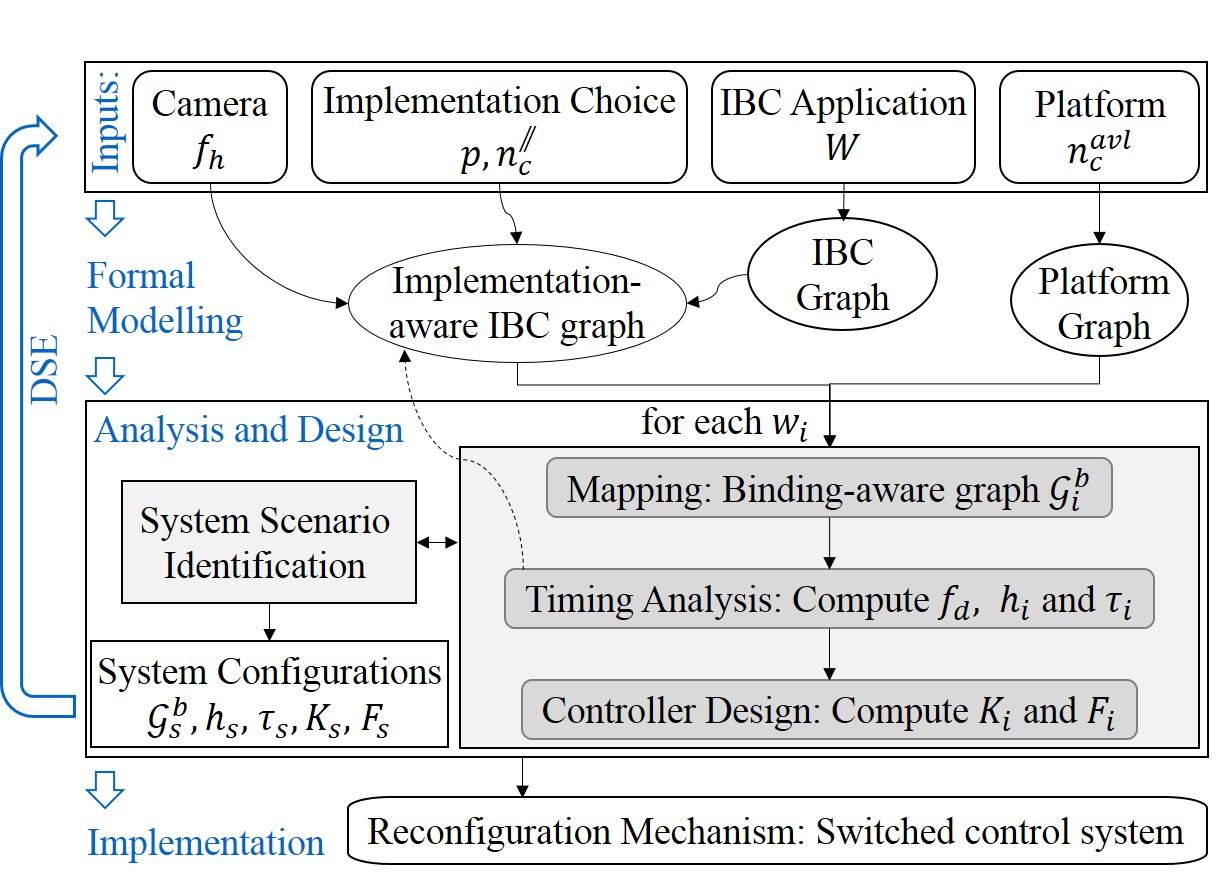
\includegraphics[width=\textwidth]{01_intro/images/SPADeOverview5.jpg}}
%\vspace{-1ex}
\caption{Overview of our \gls{spade} design flow for pipelined parallelism. $\setW$ is the set of varying workloads and $\aWorkload_i,\ \bindingAwareSDFG{i},\ \tau_i,\ h_i, \Kgain_i$ and $\Fgain_i$ are the workload, binding-aware graph, sensor-to-actuator delay, sampling period, feedback gain and feedforward gain for a workload scenario $s_i$ (determined by $\aWorkload_i\in \setW$); 
$\bindingAwareSDFG{s},\ \tau_s,\ h_s, \Kgain_s$ and $\Fgain_s$ are the corresponding parameters for an identified system scenario $s_s$ (that abstract multiple workload scenarios). $\fh$ is the camera frame arrival period, $\fd$ is the inter-frame dependence time, $p$ is the number of pipes for pipelining, $\numCoresParallel$ is the number of cores allocated for parallelism per pipe, and $\numCoresAvailable$ is the total number of available cores. For the scope of the thesis, the pipelined implementation is always periodic.}
\label{fig:ch1_spade_overview}
%\vspace{-1em}
\end{figure}
\begin{enumerate}
    \item Formal modelling of the \gls{ibc} system: An \gls{ibc} application is captured as an \gls{ibc} \gls{sadf} considering workload variations $\setW$ and the platform as a platform graph. Further, an \emph{implementation-aware} \gls{ibc} \gls{sadf} captures the given design parameters - camera frame arrival period $\fh$, maximum number of allowed pipes $\numPipes$, total number of available cores $\numCoresAvailable$ and allocated processing cores for parallel execution per pipe $\numCoresParallel$.
    The design parameters fully determine the implementation choice - non-pipelined without parallelism, non-pipelined with parallelism, pipelined without par\-al\-lelism and pipelined with parallelism. The parallelism here refers to the parallel execution of sensing subtasks limited by the degree of parallelism of the \gls{ibc} application.
    \item Analysis and design: We map the implementation-aware \gls{ibc} graph for each workload $\workloadScenario \in \setW$ to the platform graph to obtain the \emph{binding-aware graph} $\bindingAwareSDFG{i}$ for that specific workload using the SDF3 mapping flow~\cite{stuijk2007}. 
    $\bindingAwareSDFG{i}$ is a \gls{sdfg} that models the mapping of the implemen\-tation-aware graph to the platform graph. The mapping binds each actor in the \gls{sdfg} to a processing core in the platform graph. For the ordering of execution of actors bound to the same core, a static-order schedule is encoded in the \gls{sdfg}.
    A throughput and latency analysis of $\bindingAwareSDFG{i}$ yields the sensor-to-actuator delay $\tau_i$, and sampling period $h_i$.
    For a pipelined implementation, the throughput analysis of the worst-case image-workload scenario allows to compute the inter-frame dependence time $\fd$ (explained later in Section~\ref{sec:ch7_IFD}). 
    If $\fd>h_i$, the implementation-aware graph is updated with the realisable period and $\tau_i$ and $h_i$ are recomputed. 
     The controllers are then designed for the resulting $(\tau_i,\ h_i)$ to obtain the controller feedback and feedforward gains $(\Kgain_i,\ \Fgain_i)$.
     Trying to cater to the designed workload scenarios at runtime means that we have a switching system. A switching system with too many switching states is challenging for controller stability and may result in poor performance. 
     Hence, we aggregate multiple workload scenarios with similar control timing parameters as a \emph{system scenario}.
    A system scenario $\sysScenario$ abstracts multiple workload scenarios and has a constant $(\tau_s,\ h_s)$ during implementation. A \emph{system configuration} is defined as the combination of mapping and controller configurations, i.e. $\bindingAwareSDFG{s}$, $\tau_s,\ h_s,\ \Kgain_s,$ and $\Fgain_s$ (as explained later in Section~\ref{sec:ch7_sysConfigStability}).
    It should be noted that the controller gains (i.e.,  $\Kgain_s$, and $\Fgain_s$) can be designed using different approaches depending on the design goals.
    In this thesis, the \gls{spade} flow is illustrated using the \gls{lqr}, \gls{lqi}, \gls{lqg}, \gls{mpc}, and \gls{mjls} controller design approaches.
    Typically, the number of identified system scenarios is low in number, and the idea is that switching between the system scenarios at runtime guarantees stability and improved performance.
    For pipelined parallelism, a \gls{dse} using the \gls{spade} flow needs to be performed by varying the design parameters to identify the best implementation choice (parameters $\numPipes, \numCoresParallel$, further explained in Section~\ref{sec:ch7_DSE}).
    \item Runtime implementation: The system configurations for the implementation choice are stored in a \gls{lut} in platform memory for the runtime implementation. Dynamic runtime reconfiguration may be needed since there can be a switching behaviour between system configurations due to image-workload variations.
\end{enumerate}

\section{Motivating case study: \texorpdfstring{\gls{lkas}}{lkas}}
\label{sec:lkas_case_Study}
This thesis uses the motivating case study of a \gls{lkas}.
\begin{figure}
\centerline{
    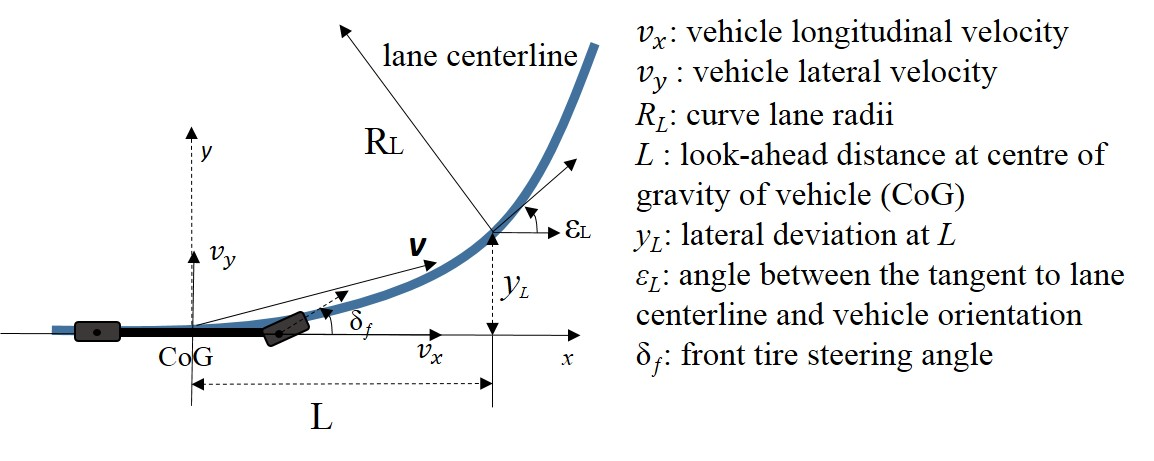
\includegraphics[width=\textwidth]{01_intro/images/model.jpg}
    }
    \vspace{-1em}
    \caption{\Gls{lkas} dynamics model derived from~\cite{kosecka1997vision}.}
    \label{fig:intro_model_lateral_control}
    %\vspace{-1em}
\end{figure}
The bicycle model derived from~\cite{kosecka1997vision} (illustrated in Fig.~\ref{fig:intro_model_lateral_control}) is considered for simulating the \gls{lkas} of a vehicle\footnote{The (default) vehicle parameters are those specified in~\cite{kosecka1997vision} for Honda Accord.} on a straight road and it is described as follows,
\begin{align*}
  \Acont (v_x)&= \left[
  \begin{array}{cccc}
    -\frac{c_{f}+c_{r}}{mv_{x}} & \frac{-mv_{x}^2+c_{r}l_{r}-c_{f}l_{f}}{mv_{x}} & 0  & 0\\
    \frac{-l_{f}c_{f}+l_{r}c_{r}}{I_{\psi}v_{x}} & -\frac{l_{f}^2c_{f}+l_{r}^2c_{r}}{I_{\psi}v_{x}} & 0 & 0\\
    -1 & -L & 0 & v_{x} \\
    0 & -1 & 0 & 0
  \end{array}
\right],\\ \Bcont &=\left[
  \begin{array}{cccc}
    \frac{c_{f}}{m} &
    \frac{l_{f}c_{f}}{I_{\psi}} &
    0&
    0
  \end{array}
\right]^{\top},\\ 
 \Ccont &=\left[
  \begin{array}{cccc}
    0 &
    0 &
    1&
    0
  \end{array}
\right], \\
\Dcont &=\textbf{0},
\end{align*}
 where, referring to Fig.~\ref{fig:intro_model_lateral_control}, we define the state vector $x(t) = [v_{y}, \dot{\psi}, \yL, \varepsilon_{L}]$, the measured output $y(t)$ as $\yL$, and the control input $u(t)$ as the steering angle $\delta_f$, where
$\dot{\psi}$ is the vehicle's yaw rate in rad/s, where the velocity components $v_x$ and $v_y$ are in m/s, where $l_{f}$,\ $l_{r}$ ($=1.22$ and $1.62$ m respectively) denote distance of the front and rear axles from the \gls{cog}, where 
$I_{\psi}$ ($=2920$ kg$\cdot$m$^2$) is the total inertia of the vehicle around its \gls{cog}, where
$c_{f}$,\ $c_{r}$ (${=1.2\times10^5\text{~N/rad)}}$ denote cornering stiffness of the front and rear tires, and where the total mass of the vehicle is $m$ ($=1590$ kg). Note that the model can be either linear time-invariant or time-variant depending on whether longitudinal velocity $v_x$ is constant or time-varying. 


\section{Thesis outline}
This thesis is organized along the research challenges and scientific contributions outlined in Section \ref{chap:challenges}. Accordingly, the five scientific contributions are reported in Chapter \ref{chap:parallelisation} to Chapter \ref{chap:approximation}. 
Chapters \ref{chap:parallelisation}, \ref{chap:pipelined} and \ref{chap:pipelined_parallelism} focus on platform-aware design aspects where the research focus has been on reducing sampling period and delay by parallel implementation (Chapter \ref{chap:parallelisation}), pipelined implementation (Chapter \ref{chap:pipelined}) or their combination (Chapter \ref{chap:pipelined_parallelism}). Chapters \ref{chap:workloadVariations} and  \ref{chap:approximation} report design approaches exploiting application-specific characteristics. Chapter \ref{chap:workloadVariations} reports the proposed approach on dealing with workload variation in a sequential \gls{ibc} implementation. Chapter \ref{chap:approximation} presents the approximation-aware design of an \gls{ibc} system. It presents the \gls{imacs} framework for approximate computing in closed-loop systems. Chapter \ref{chap:concl} makes some concluding remarks and outlines a number of relevant future extensions. 

\vfill